\documentclass{beamer}
\usepackage[size=a1]{beamerposter}
\usepackage[sfdefault]{FiraSans}
\usepackage{FiraMono}
\usepackage{hyperref}

\definecolor{oxfordblue}{RGB}{0,33,71}
\setbeamercolor{background canvas}{bg=oxfordblue}
\setbeamercolor{normal text}{fg=white}
\usebeamercolor[fg]{normal text}
\setbeamertemplate{navigation symbols}{}

\setlength{\parskip}{2\baselineskip}

\begin{document}
\begin{frame}
  \begin{columns}[c]
    \begin{column}{.85\textwidth}
      \centering\VERYHuge\url{https://github.com/nicolaspayette/qual2rule}
    \end{column}
    \begin{column}{.1\textwidth}
      
\includegraphics[width=\linewidth]{ox_brand_cmyk_rev.pdf}
    \end{column}
  \end{columns}
  \vfill
  \begin{center}
    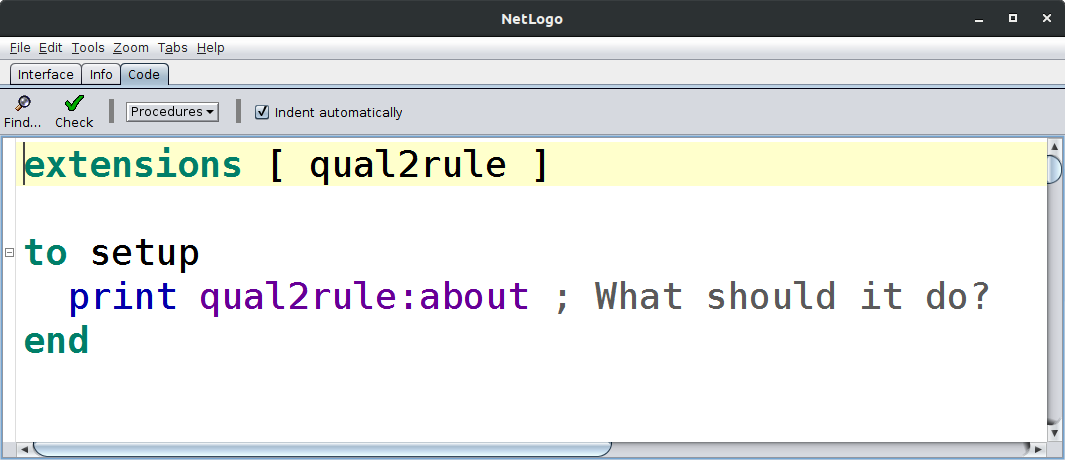
\includegraphics[height=0.35\paperheight]{screenshot}
    \vfill
    \VERYHuge Please take a short survey!\par
    
\includegraphics[height=0.2\paperheight]{qr-code}\par
    \LARGE\url{https://forms.gle/dsXoAD3zLXonbpSU9}
  \end{center}
\end{frame}
\end{document}
